\chapter{Methods}
In the present chapter, the general methodology and approach chosen for the validation of the NWCSAF CI product is presented.

\section{Validation region and parallax correction}
The validation region of this study is defined by the standard domain of the German weather radar network as given in \citet{RADOLANkurz2018}, which spans \SI{900 x 900}{\kilo\metre} with a spatial resolution of \SI{1 x 1}{\kilo\metre}. All satellite observations and products have been interpolated to this grid using nearest neighbour interpolation.

The slanted viewing angle of Meteosat SEVIRI for Central Europe causes an apparent shift of cloud fields in the satellite imagery. This shift depends on the cloud-top height and is mainly in northward direction for our viewing geometry. The effect is called "parallax effect" and typically leads a mismatch between radar-derived convective precipitation data (which do not suffer from such a shift) and the satellite imagery. If we look at combined cloud-precipitation-structures at the kilometer-scale, the parallax shift is of similar magnitude and  can not be ignored. Hence, a geometric transformation of the satellite fields has to be applied to correct for this effect.

As mentioned above, Meteosat SEVIRI data and NWCSAF products have been reprojected onto the radar grid with an approximative grid spacing of one kilometer. This fine grid ensures that no information from satellite observations is lost in the data combination. Now, the task of the parallax transform is to reproject the satellite data in such a way that cloud fields and structures appear like being sensed from a (hypothetical) nadir viewing platform. This ideal transformation is however hard to achieve because of several issues:
\begin{itemize}
\item \textbf{semi-transparency of multi-layer problem:} For semi-transparent or multi-layer clouds it is hard to assess where directly radiation comes from. That might also differ from channel to channel and not enough information is in the satellite data to reconstruct the cloud field three-dimensionally and independently apply shifts of separate layers.
\item \textbf{spatial resolution problem:} Cloud-top height estimates are needed for parallax correction. These are typically derived from narrow-band, but "coarse" resolution infrared channels. For some of the applied cloud-top height methods, the spatial resolution is even coarser than the standard Meteosat pixel resolution. Therefore, it can not be expected that the cloud texture information is meaningfully contained in the cloud-top height product. 
\item \textbf{information loss:} An ideal parallax correction would remove information obtained from the cloud-side observation. This information would be lost and holes in the images would appear behind the cloud towers where no remote sensing signal is available.
\end{itemize}
With these issues in mind, we choose the following strategy for applying a parallax transform:
\begin{enumerate}
\item Cloud-top height products have been calculated. For simplicity, we chose the TROPOS cloud product production chain that is based on NWCSAF version 2013 using ECMWF forecasts as numerical simulation.
\item Cloud-top height products have been smoothed. The reason for the smoothing choice is that sharp edges in the cloud-top height product destroy the texture of the parallax-corrected satellite images and introduces unwanted artifacts into the results. We choose a sequence of two filters: first a percentile filter based on the 90-th percentile with a footprint of 21 km, second a convolution filter with a Gaussian kernel of 9 km width.
\item Parallax-corrected latitude and longitude positions of clouds have been calculated based on the source code provided by the NWCSAF team.
\item The new lat-lon positions define a distortion of the original grid. We use a readily available image warping algorithm which utilizes cubic interpolation to remap the distorted grid onto the radar grid (the skimage.transform.warp function provided by the Scikit-Image Python library)  
\end{enumerate}

\begin{figure}[!b]
\centering
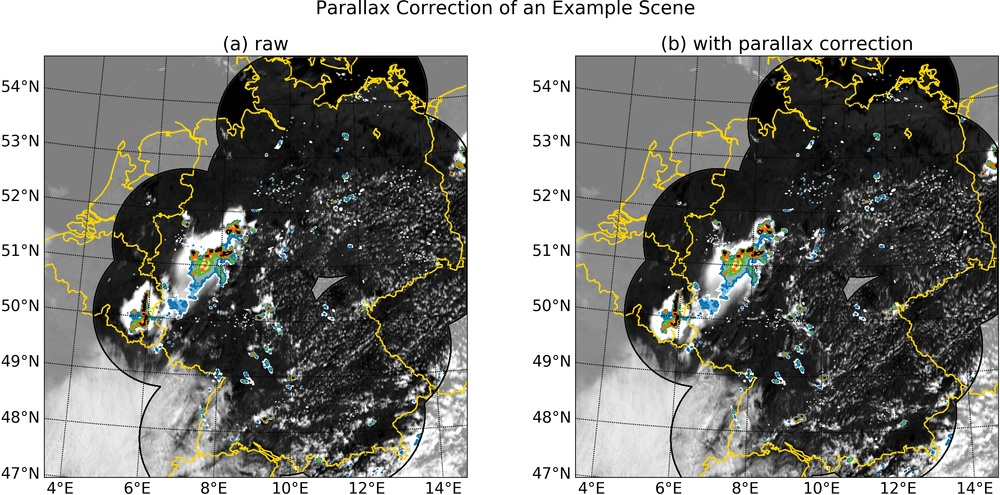
\includegraphics[width=\textwidth]{Grafiken/Abbildungen/parallax_example.jpg}
\caption{An example scene for a combination of Meteosat SEVIRI HRV reflectances (gray shades) and Radolan RX radar reflectivities (colored shades) for 23 May 2012, 12:30 UTC . (a) Raw combination of regridded data and (b) combination of data with HRV reflectance being parallax corrected. Coastline and country borders are in yellow, region with no radar coverage has been masked out with gray overlays.}
\label{fig:parallax_example}
\end{figure}
An example of the parallax transform applied to the HRV reflectances is shown in Fig.~\ref{fig:parallax_example}. The image transformation significantly improves the overlap between radar-derived precipitation signatures and cloud features. Some distortion of the cloud fields is still visible, we however consider the result of the parallax transform method as a good compromise. 


\section{Definition of Ground Truth}
\label{sec:haci}
Using the RADOLAN RX composite, isolated convective objects have been identified using the method described in \citet{Haberlie_2015}. First the radar data (Fig.~\ref{fig:haberlie}a) has been masked using a reflectivity factor threshold of \SI{35}{\dbZ} (Fig.~\ref{fig:haberlie}b) to delineate convectively active regions. These regions are then grouped into objects by requiring connectivity. A buffer mask is generated around existing objects as well as the border of the radar range using a buffer radius of \SI{15}{\kilo\metre}. This buffer mask is applied to the next time step, in order to identify newly developing convective objects (Fig. \ref{fig:haberlie}c). Finally, all newly developed convective objects outside the buffer mask with a reflectivity factor of over \SI{35}{\dbZ} are considered as new convective objects, which have thus initiated within the last five minutes (Fig.~\ref{fig:haberlie}d). Requiring a minimum object life time of \SI{30}{\minute} together with some additional  criteria, only objects are retained which have a sufficient life time to be considered as convective objects (Fig.~\ref{fig:haberlie}e). Convective object identification is done at five minutes time resolution for all case days, and is subsequently aggregated to \SI{15}{\minute} time steps to match the temporal resolution of the NWC\,SAF CI product. These object represent the ground truth used further for the validation of the CI product.

\begin{figure}[htbp]
\centering
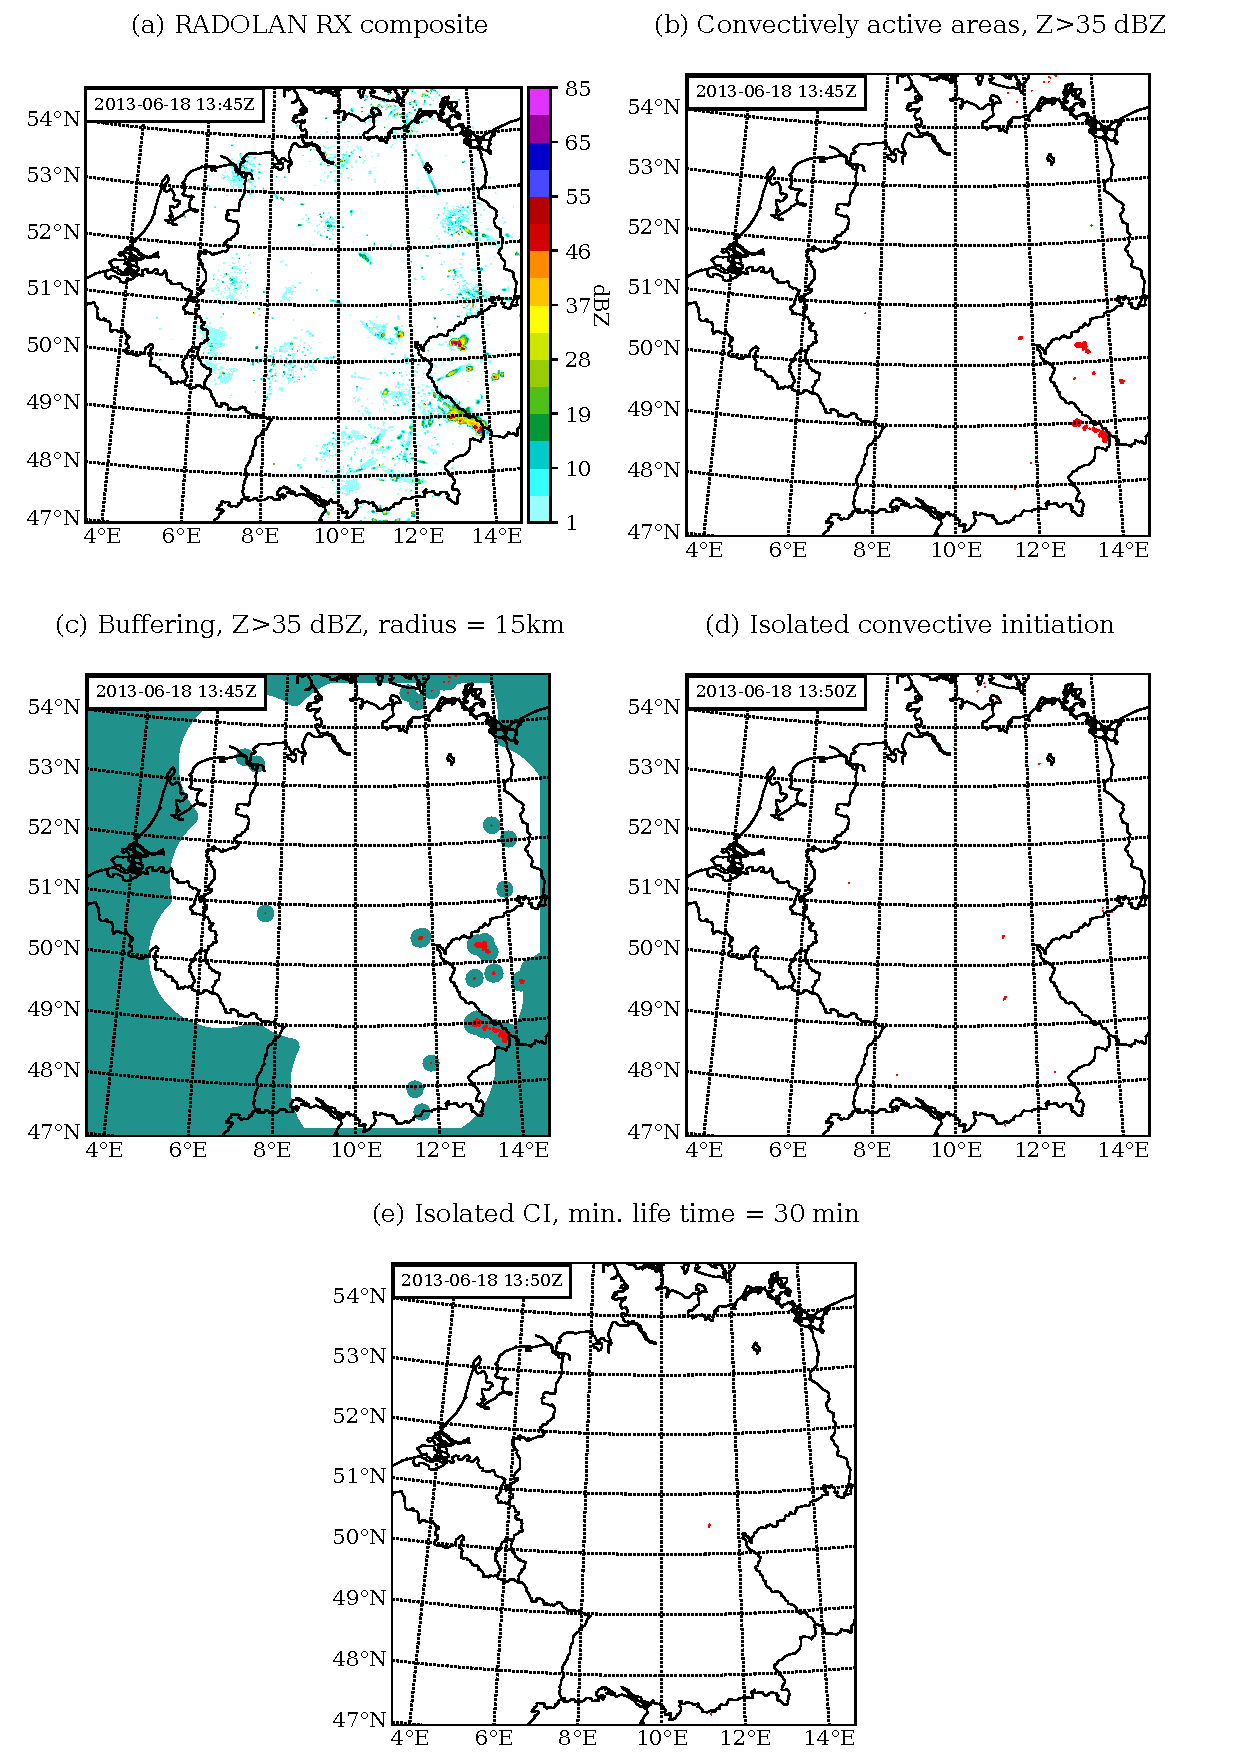
\includegraphics[height=\textheight]{Grafiken/Abbildungen/haberlie_prinzip.pdf}
\caption{Principle of deriving the ground truth. Using weather radar data (a), the data are masked using a reflectivity threshold of \SI{35}{\dbZ} to derive convectively active areas (b). Then these objects are buffered using a buffer radius of \SI{15}{\kilo\metre} (c). Using these buffers the, data of the next time step is masked, so that only isolated newly developing convection is taken into account (d). After that, to only consider precipitating objects with an adequate life  time, all objects with a minimum life time below \SI{30}{min} are masked out (e).}
\label{fig:haberlie}
\end{figure}

It has to be noted that this definition of ground truth is rather strict and quite different from the approach chosen by \citet{Karagiannidis2016}.  

\section{Derivation of motion fields}
The motion of cloud fields in the satellite observations was estimated using the implementation of the TV-L1 optical flow algorithm proposed by \citet{Zach2007}. The Python interface to the OpenCV library \citep{opencV_library} has been used here. The algorithm parameters selected here where optimised using the MPI Sintel test dataset \citep{Butler:ECCV:2012}, and are given in Tab. \ref{tab:oflow}. Motion fields have been calculated from Meteosat's IR \SI{10.8}{\micro\metre} and HRV channels considering \SI{15}{\minute} time steps. 
The TV-L1 optical flow approach differs from the cross correlation-based approach by MecikalskiBedka2006 to derive atmospheric motion vectors (AMV) by allowing discontinuities in the flow field, and tends to be more robust against noise than other techniques of motion tracking Perez2013.

\begin{table}[htb]
\caption{opencv parameters used for the estimation of the optical flow using the method proposed \citet{Zach2007}}
\begin{tabular}{llS} 
\toprule
parameter & description & {value}\\ 
\midrule 
$\epsilon$ & stopping criterion threshold used in the numerical scheme & \num{0.01}\\ 
$\gamma$ & coefficient for additional illumination variation term & 0.4\\ 
$\lambda$ & weight parameter for the data term, attachment parameter & 0.2\\ 
$\mu$ & kernel size of the median filter & 1\\ 
$\tau$ & time step of the numerical scheme & 0.25\\ 
$\theta$ & Weight parameter for (u - v)\textsuperscript{2}, tightness parameter & 0.8\\ 
$\mathrm{N}_\mathrm{inner}$ & number of inner iterations  used in the numerical scheme & 7\\ 
$\mathrm{N}_\mathrm{outer}$ & number of outer iterations  used in the numerical scheme & 40\\ 
$\mathrm{N}_\mathrm{scales}$ & number of scales used to create the pyramid of images & 5\\ 
$\mathrm{S}_\mathrm{scales}$ & steps between scales & 0.5\\
$\mathrm{N}_\mathrm{warp}$ & number of warpings per scale & 5\\ 
\addlinespace
\bottomrule
\end{tabular}
\label{tab:oflow}
\end{table}

\section{Cloud objects}
\label{sec:cloud}
To validate the detections of the NWC\,SAF CI product and the detections of the radar based approach presented above, cloud objects have been derived. 

The cloud objects are based on the NWC\,SAF cloud mask product and the MSG HRV channel, as its higher spatial resolution allows for a better separability of cloud objects than the standard MSG resolution. As the HRV channel is in the visible spectrum, and so there is no data for the night time, only a time frame of twelve hours centered around noon CET (05:00 am UTC to 05:00 pm UTC) has been chosen for the derivation of cloud objects. This time frame has the advantage that there is data for all case days and it also avoids the time around sunrise and sunset where atmospheric scattering effects make the data not usable for our objective.

For the derivation of meaningful cloud objects, the rather high HRV spatial resolution also has the drawback that often very small non-convective clouds are derived as cloud objects leading to an artificially high rate of missed detections. To overcome this, the HRV field (Fig.~\ref{fig:hrv_seg}a) was filtered using a Gaussian filter (Fig.~\ref{fig:hrv_seg}b) and the objects were derived from the smoothed HRV field (Fig.~\ref{fig:hrv_seg}c and d). Additionally a minimum size an object has to have to be considered was set. To find suitable filter, minimum size and threshold parameters, a number of different parameters combination has been tested against the overlap size of ground truth objects and cloud objects for the 25\textsuperscript{th} May 2010. The result of the analysis is shown in Fig. \ref{fig:filter-parameters}. It turns out, that the two parameters with the highest impact on the overlap size are the size of the Gaussian kernel and the threshold used to define which parts of the HRV channel field are objects. The minimum size of the objects and the connectivity used to segment the objects does not seem to have a large influence. The maximum intersection size between ground truth and cloud objects can be achieved by a rather strong smoothing, setting the Gaussian filter parameter \textsigma~to 3, and setting the HRV threshold to \num{0.3}. Additionally, for the derivation of the cloud objects, to avoid too small objects, the minimum object size was set to \num{10} \SI{1x1}{\kilo\metre} pixels and the connectivity type to \num{8} neighbours. 
 
\begin{figure}[htbp]
\centering
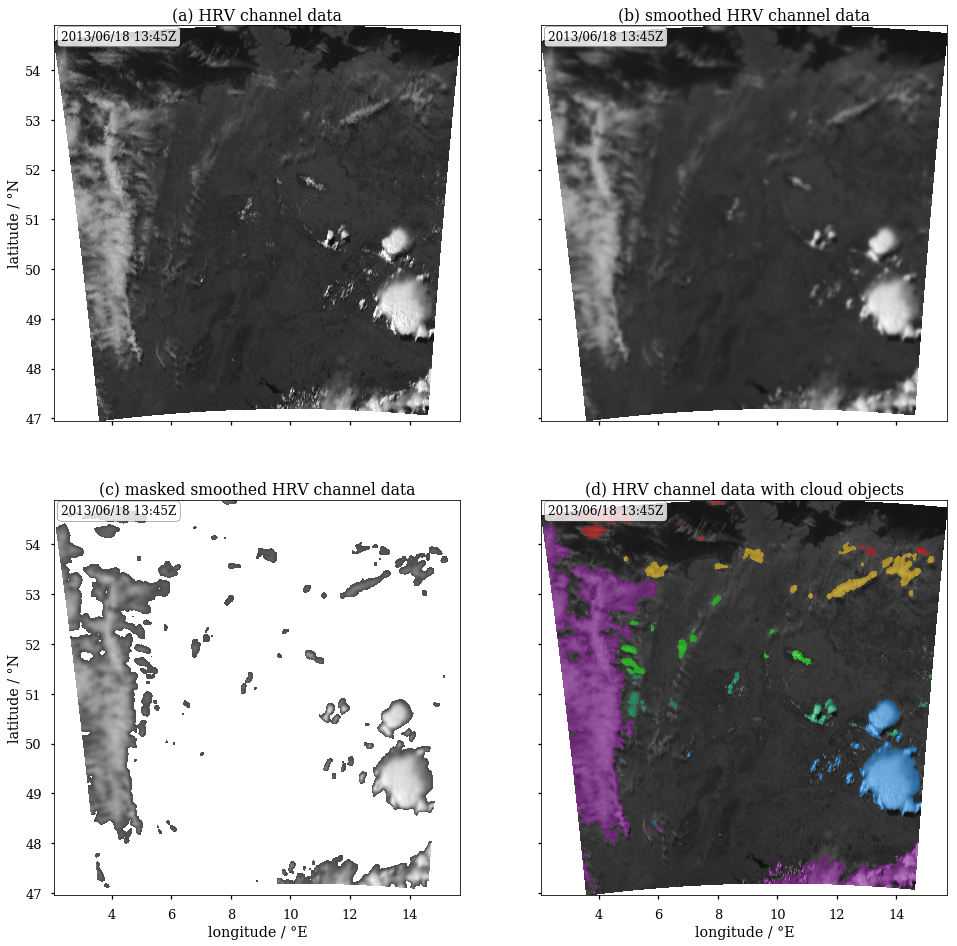
\includegraphics[width=\textwidth]{Grafiken/Abbildungen/wolkenobjektprinzip.png}
\caption{Principle of deriving the cloud objects. Using HRV channel data (a), the data are smoothed using a Gaussian blur filter with a \textsigma~value of 3 (b). Then these objects are buffered using a buffer radius of \SI{15}{\kilo\metre} (c). Using these buffers, the, data of the next time step is masked, so that only isolated newly developing convection is taken into account (d). }
\label{fig:hrv_seg}
\end{figure}

\begin{figure}[htbp]
\centering
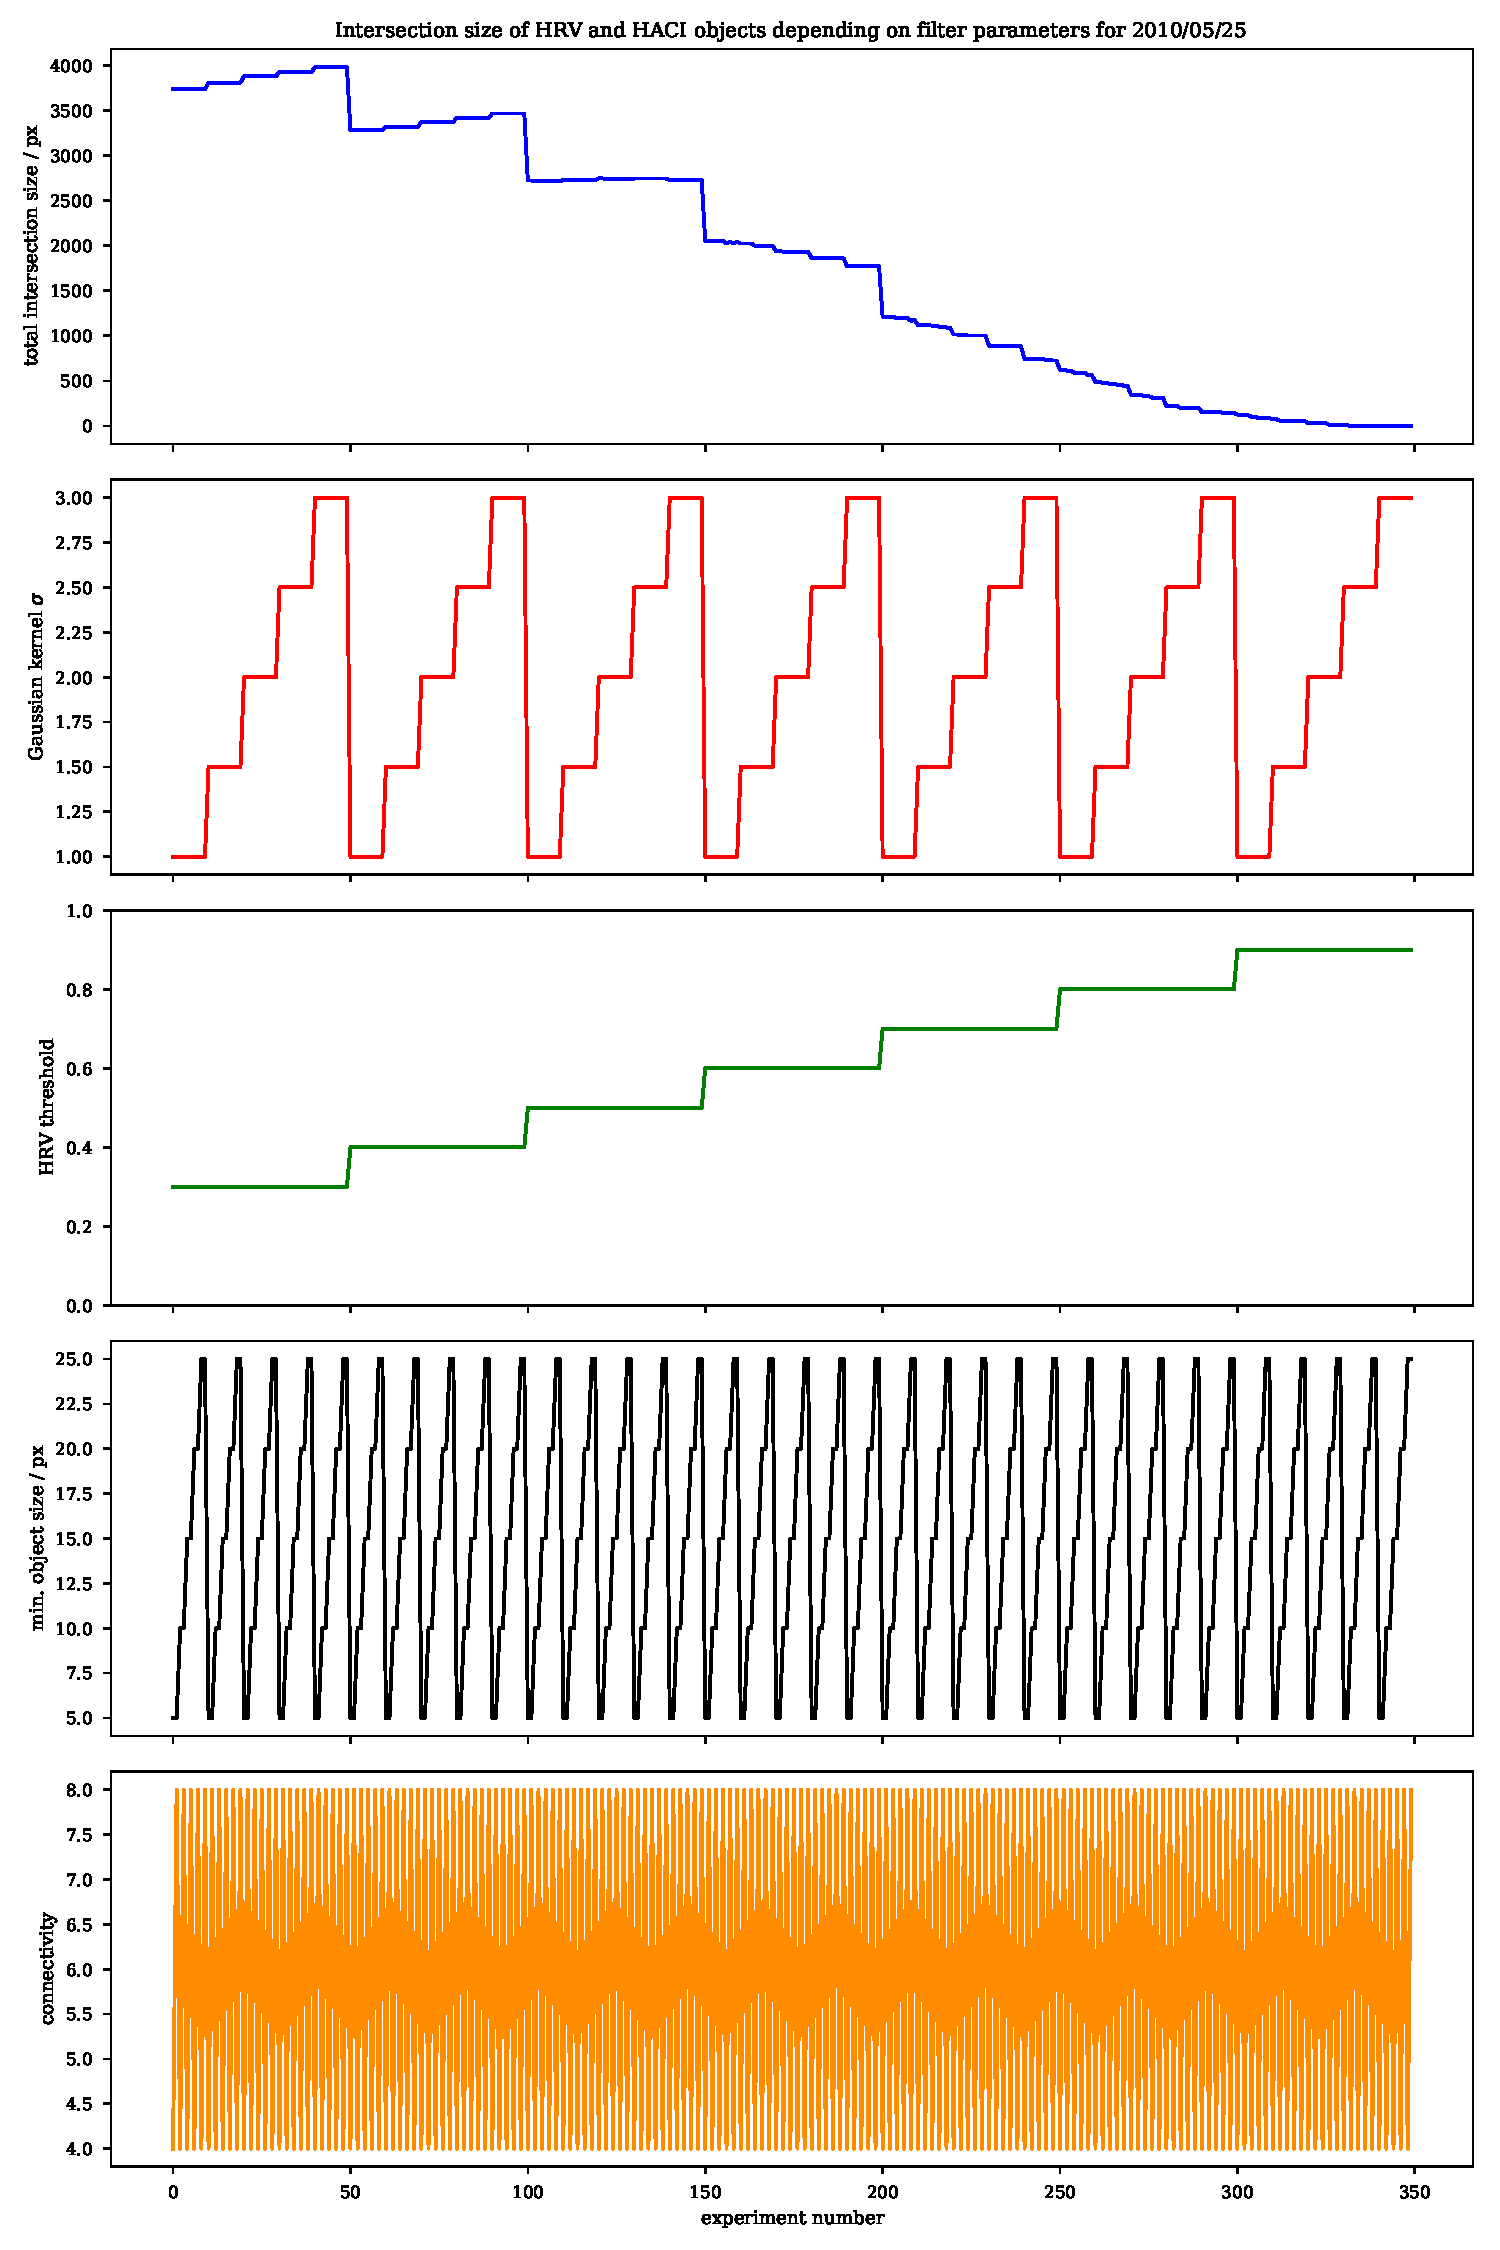
\includegraphics[height=\textheight]{Grafiken/Abbildungen/parameter_plot.pdf}
\caption{Intersection size (top most figure) between cloud and ground truth objects for combinations of four filters and segmentation parameters (figures below).}
\label{fig:filter-parameters}
\end{figure}

Objects tracks are created using the motion fields derived from the MSG HRV channel applying an overlap tracking approach. Starting from the first emergence of the particular object, the object is moved forward in time using the motion field. If the objects of the first and second time step overlap, an object path is created for the two time steps and so on. As the object structure often is quite complex with many splits and merges, mathematical graphs have been created to allow for an analysis of the object structure. Using the graphs, only single cell objects the part of the object tracks prior to splits and merges have been used in the further analysis. To allow for a comparison with the radar data, the tracks also have been parallax corrected using the cloud top height of the NWC\,SAF cloud height product.

To be consistent with the ground truth definition, only objects with a minimum life time of \SI{30}{\minute} have been considered in the further analysis.

\section{Validation approach}
\label{sec:validation}
The validation of the NWC\,SAF CI product  is based on cloud objects derived from MSG HRV data and weather radar detections as ground truth.

As shown in Fig. \ref{fig:schema}, the validation strategy is based on the intersection of cloud objects, detectrions by the CI product and ground truth objects. Given a track of a cloud object the cloud object is considered to be detected by the NWC\,SAF CI product if there is an intersection between the cloud object and pixels with a CI probability of strictly larger than \SI{0}{\percent}. If there is an intersection between the cloud object and pixels with different CI probabilities for one time step, only the highest CI probability is counted, and if there are more than one intersections of the cloud object and CI pixels along the object track, only the first intersection time step is counted. 

In the next step, starting from the CI detection time step, it is checked if there is an intersection between the cloud object and a ground truth object within the next \SI{30}{\minute}. If necessary, the track is getting extended by propagating the last available track point forward in time using the motion fields. If an intersection between a detected cloud object and a ground truth object can be observed within the next \SI{30}{\minute} it is counted as a true positive case for the highest CI probability level of the detection time step. If not, than it is counted as a false positive case.

If there are intersections with at least one ground truth object along the cloud object track and there are no intersections with CI pixels or the intersection with the first intersection with a ground truth object is earlier than the first intersection with CI pixels, the case is counted as false negative.

If a cloud object neither intersects with CI pixels nor with a ground truth objects it is counted as true negative.

The validation is performed separately for all CI levels. The confusion matrix of the validation approach is given in Tab.~\ref{tab:confusion}.

\begin{figure}[htbp]
\centering
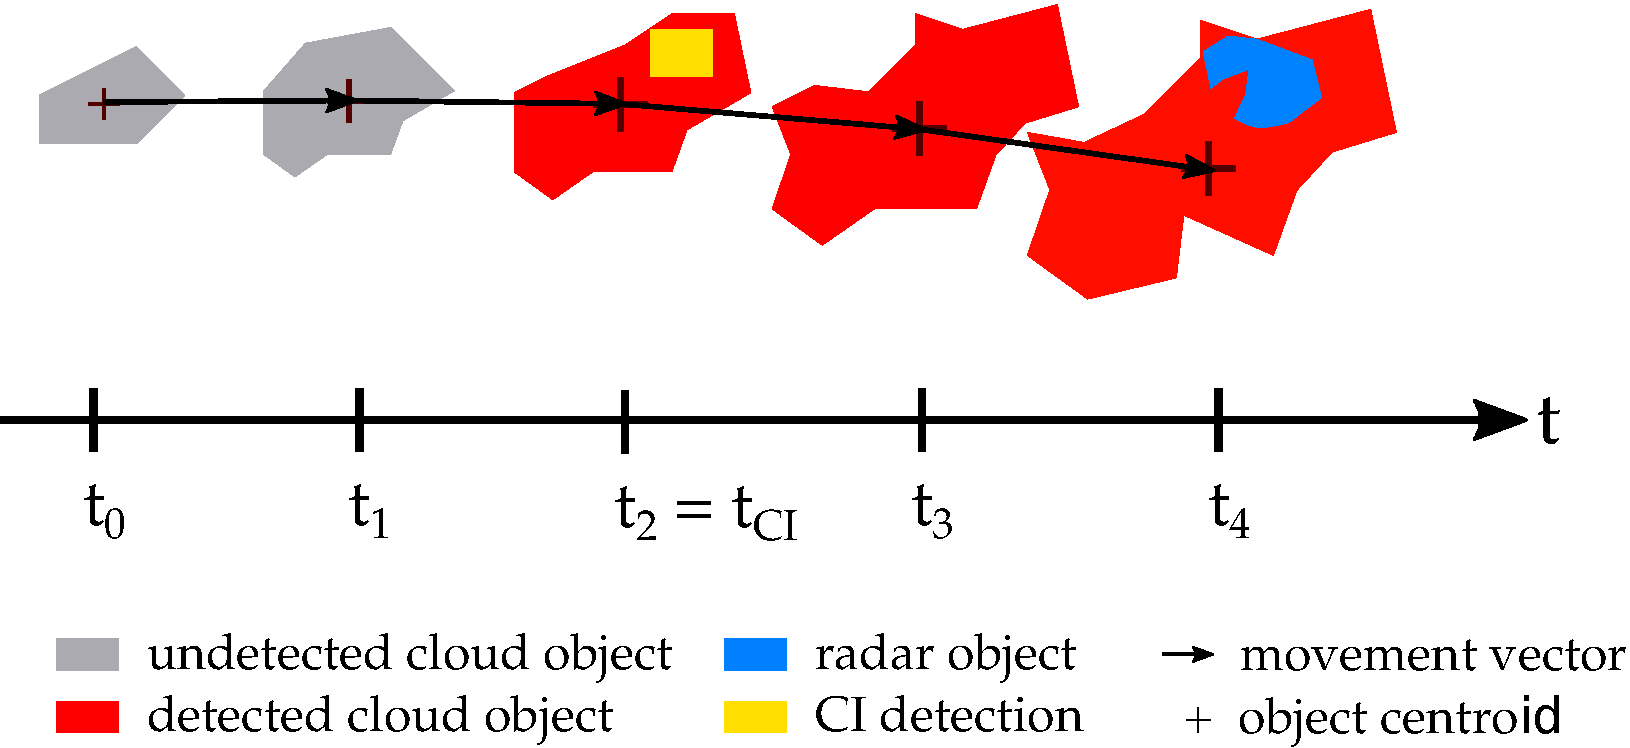
\includegraphics[width=0.9\textwidth]{Grafiken/Abbildungen/verification_scheme_new.pdf}
\caption{Schematic of the validation approach. Starting from a cloud object (grey and red) a cloud object track is created (denoted by the vector arrows) . If a CI object (yellow) is inside the validation area a new object track with validation region is created. If a radar object (blue) is detected inside the new \SI{30}{\minute} validation area the cloud object is counted as a true positive}
\label{fig:schema}
\end{figure}

\begin{table}[htbp]
\centering
\caption{Confusion matrix for the validation, TP = true positive, FP = false positive, FN = false negative, TN = true negative}
\begin{tabular}{cccc} 
\toprule
{CI product detection} & \multicolumn{2}{c}{weather radar detection} \\
					   \cmidrule{2-3}
					   & yes  & no \\
\midrule
yes                    &  TP  & FP \\
no                     &  FN  & TN \\ 
\addlinespace
\bottomrule
\end{tabular}
\label{tab:confusion}
\end{table}

For the assessment of the validation, several metrics can be derived from the confusion matrix. In this study the following are used:

\begin{itemize}
\item Probability Of Detection $\mathrm{POD} = \frac{\mathrm{TP}}{\mathrm{TP} + \mathrm{FN}}$, which is the probability to detect an event
\item False Alarm Ratio $ \mathrm{FAR} = \frac{\mathrm{FP}}{(\mathrm{FP} + \mathrm{TP})} $, which is a measure for the fraction of forecast that do not become events
\item Heidke Skill Score \citep{Heidke1926} $\mathrm{HSS} = \frac{2 (\mathrm{TP} \cdot \mathrm{TN}) - \mathrm{FP} \cdot \mathrm{FN}}{ (\mathrm{TP} + \mathrm{TF}) (\mathrm{FN} + \mathrm{TN}) (\mathrm{FP} + \mathrm{TN})}$, which is a measure of how good is the algorithm performance against a detection by chance
\item Critical Sucess Index $ \mathrm{CSI} = \frac{\mathrm{TP}}{\mathrm{TP} + \mathrm{FN} + \mathrm{FP}}$, which is a measure of how well forecasts events correspond to observed events 
\end{itemize}